\chapter{Appendix | Advertisement Logger's Implementation} \label{AppendixC}

\section{Scanning \gls{ble} Advertisements}

According to the Bluetooth 4.0 Core specifications, an advertisement event consists of an advertising device periodically send advertisement packets. The interval of these advertising events can range from 20 ms to 10 s. In each of these advertising events an advertiser sends an advertising packet in each channel in an interval of 10 ms starting with channel 37. The objective of a BLE advertisement scanner would be to be able to receive the packets from at least one channel in an advertisement event, while saving power. To achieve this trade off, the radio duty cycles between receiving and disabled state, while being in the next advertising channel every time it is switched on. The total time of this periodic event is known as the \emph{Scan Interval}, while the time the radio is on is known as \emph{Scan Window}. The figure\footnote{https://devzone.nordicsemi.com/question/2535/what-is-the-minimum-time-for-a-app-and-a-peripheral-to-create-a-connection/} \ref{fig:AdvScanBLE} depicts this process.

\begin{figure}[h]
\centering
\includegraphics[width=\textwidth]{AdvScanBLE}
\caption{Scanning BLE advertisements}
\label{fig:AdvScanBLE}
\end{figure}

\section{Software Architecture}
The following flow charts explain the software architecture of the \emph{Advertisement Logger}.
\subsection{Main Function}
The execution of the program starts with the main function after reset as depicted by figure \ref{fig:main_chart}. Note that the radio is initialized to continuously receive packets once it has started while also measuring the received signal strength \acrshort{rssi}.
\begin{figure}[h]
\centering
\vspace{80pt}
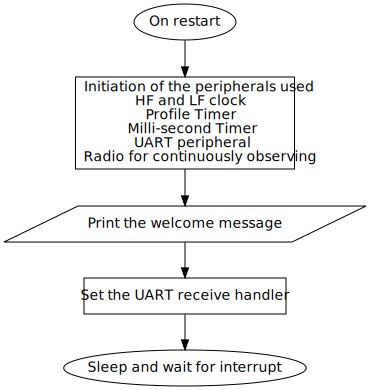
\includegraphics[scale=0.85]{main_chart}
\caption{Main function flowchart}
\vspace{80pt}
\label{fig:main_chart}
\end{figure}

\subsection{UART String Receive Handler}
The UART String Receive handler which gets a string sent to the \gls{soc} through an unsigned character pointer checks if the string is either \texttt{START} or \texttt{STOP} so that the scanning of the advertisements can be started or stopped respectively.
\begin{figure}[h]
\centering
\vspace{50pt}
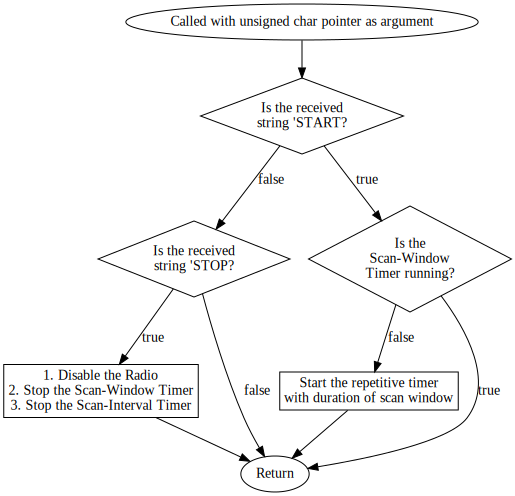
\includegraphics[scale=0.85]{UartISR_chart}
\caption{UART string receive handler flowchart}
\vspace{51pt}
\label{fig:UartISR_chart}
\end{figure}
\clearpage

\subsection{Scan Interval Timer Handler}
The scan interval timer is a repetitive timer with an interval equal to the scan interval. At the beginning of the scan interval this function performs 5 different tasks as shown in figure \ref{fig:scanInterval_chart}.
\begin{figure}[h]
\centering
\vspace{20pt}
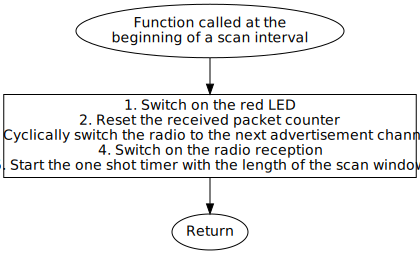
\includegraphics[scale=0.85]{scanInterval_chart}
\caption{Scan interval timer handler flowchart}
\label{fig:scanInterval_chart}
\end{figure}

\subsection{Scan Window Timer Handler}
The scan window timer is a single shot timer with an interval equal to the scan window. At the end of the scan window this function performs 3 different tasks as shown \ref{fig:scanWindow_chart}.
\begin{figure}[h]
\centering
\vspace{20pt}
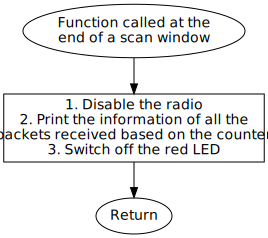
\includegraphics[scale=0.85]{scanWindow_chart}
\caption{Scan window timer handler flowchart}
\label{fig:scanWindow_chart}
\end{figure}

\subsection{Radio Interrupt Routine}
The radio peripheral is configured such that the end of a packet and the end of \acrshort{rssi} measurement trigger the interrupt. At the end of a packet, the packet's data is collected if there is space in the buffer. At the end of the \acrshort{rssi} measurement the \acrshort{rssi} value is saved.
\begin{figure}[h]
\centering
\vspace{10pt}
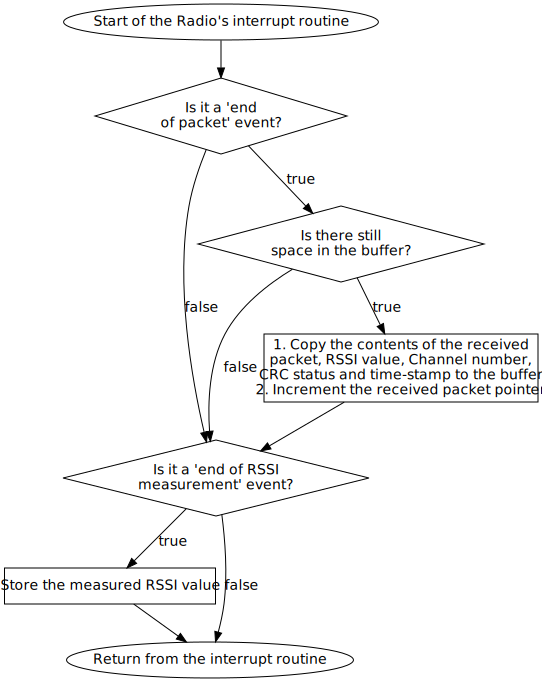
\includegraphics[scale=0.85]{RadioISR_chart}
\caption{Radio interrupt routine flowchart}
\label{fig:RadioISR_chart}
\end{figure}

\chapter{Appendix | \gls{ble} \gls{soc} Comparison} \label{AppendixA}
The dense table in the next page compares many different parameters of the \gls{ble} \glspl{soc} available. This table was compiled in the first half of 2014. Because of the high pace at which the industry around \gls{ble} is progressing, many details here might not be accurate as time progresses.

The legend for the table is

\vspace{10pt}
NA \hspace{10pt}: The information is not available

- \hspace{22pt}: The feature is not available

\includepdf[pagecommand={\begin{tikzpicture} [remember picture,overlay] \node at (7.4,-17) {}; \end{tikzpicture}},page=1]{BLE_SoCs.pdf}

\chapter{Appendix | Data Acquired} \label{AppendixB}

The entire data acquired and results computed for both High-Throughput test and Request-Response test can be found in the tables in the following pages.

%\includepdf[landscape]{HT.pdf}
%
%\includepdf[landscape]{RR.pdf}